\documentclass[10pt]{beamer}

\usepackage{textpos}
\usepackage{tikz,calc}

\usepackage[english]{babel}
\usepackage{multicol}
\usepackage{float}
\usepackage{multirow}
\restylefloat{table}
\usepackage{graphics}
\usepackage{multimedia}
\usepackage{times}
\usepackage{graphicx}
\usepackage{epstopdf}
\usepackage{epsfig}
\usepackage{epsf}
\usepackage{rotating}
\usepackage[bf,SL,BF]{subfigure}
\usepackage{verbatim}
\usepackage{amsmath}
\usepackage{paralist}
\usepackage{amsfonts,amsthm,amssymb}
\usepackage{colordvi}
\usepackage{color}
\usepackage{setspace}
\usepackage{latexsym,wasysym,mathrsfs}

\DeclareGraphicsExtensions{.pdf,.png,.jpg,.eps,.ps,.jpeg}

\usetheme{Copenhagen}

%% position the logo
%\addtobeamertemplate{frametitle}{}{%
%\begin{textblock*}{100mm}(\textwidth,-0.85cm)
%\includegraphics[height=0.8cm,width=0.8cm,keepaspectratio]{OSU_vertical_2C_O_over_B.png}
%\end{textblock*}}

% Useful commands
\newcommand{\bes}{\begin{equation*}}
\newcommand{\ees}{\end{equation*}}
\newcommand{\beq}{\begin{equation}}
\newcommand{\eeq}{\end{equation}}
\newcommand{\barr}{\begin{array}}
\newcommand{\earr}{\end{array}}
\newcommand{\Pb}{\mathbb P}
\newcommand{\E}{\mathbb E}
\newcommand{\R}{\mathbb R}
\newcommand{\N}{\mathbb N}
\newcommand{\Z}{\mathbb Z}
\newcommand{\Com}{\mathbb C}
\newcommand{\la}{\langle}
\newcommand{\ra}{\rangle}
\newcommand{\mA}{\bf A}
\newcommand{\mB}{\bf B}
\newcommand{\mC}{\bf C}
\newcommand{\ve}{\varepsilon}
\newcommand{\lar}{\leftarrow}
\newcommand{\lla}{\longleftarrow}
\newcommand{\rar}{\rightarrow}
\newcommand{\lra}{\longrightarrow}
\newcommand{\Rar}{\Rightarrow}
\newcommand{\Lra}{\Longrightarrow}
\newcommand{\oo}{\infty}
\newcommand{\si}{\sigma}
\newcommand{\prt}{\partial}
\newcommand{\ka}{\kappa}
\newcommand{\Gset}{\mathcal G}
\newcommand{\J}{\mathcal J}
\newcommand{\mO}{\mathcal O}
\newcommand{\D}{\mathcal D}
\newcommand{\x}{\sf x}
\newcommand{\z}{\sf z}
\newcommand{\risk}{\mathcal{R}}
\newcommand{\Hyp}{\mathscr{H}}
\newcommand{\Ls}{\mathscr{L}^2}
\newcommand{\im}{{\tt i}}
\newcommand{\epty}{\bigcirc\hspace{-2.5mm}\big\slash}
\newcommand{\diag}{\operatorname{diag}}
% ***** Commands for theorems *****
\theoremstyle{plain}
\newtheorem*{lma}{Lemma}
\newtheorem*{thm}{Theorem}
\newtheorem{theorema}{Theorem}[section]
\newtheorem{lema}[theorem]{Lemma}
\newtheorem{cor}[theorem]{Corollary}
\newtheorem{prop}[theorem]{Proposition}
\theoremstyle{definition}
\newtheorem*{ack}{Acknowledgments}
\newtheorem{examp}[theorem]{Example}
\newtheorem{exercise}[theorem]{Exercise}
\newtheorem{defn}[theorem]{Definition}
\newtheorem{defs}{Definition}
\theoremstyle{remark}
\newtheorem{remark}[theorem]{Remark}
\newtheorem{convention}[theorem]{Convention}
\newtheorem{statement}[theorem]{Statement}
\newtheorem{facts}[theorem]{Fact}
\newtheorem{axiom}[theorem]{Axiom}

\usepackage{pgf,tikz}
\usepackage{mathrsfs}
\usetikzlibrary{arrows}
\usetikzlibrary{matrix}
%NEW TIKZ COMMANDS
%\usepackage{verbatim}
%\usepackage[active,tightpage]{preview}
%\PreviewEnvironment{tikzpicture}
%\setlength{\PreviewBorder}{10pt}%
\usetikzlibrary{calc}
\usepackage{amssymb}

\usepackage[weather]{ifsym}

%Empty header
\makeatletter
    \newenvironment{withoutheadline}{
        \setbeamertemplate{headline}[default]
        \def\beamer@entrycode{\vspace*{-\headheight}}
    }{}
\makeatother

\setbeamertemplate{theorems}[numbered]

% Presentation parameters
\title[FMDV in African Buffalo]{FMDV in African Buffalo\\Influence of immunity in the spread 
of wildlife diseases}
\author[Ricardo Reyes]{Ricardo No\'e Gerardo Reyes Grimaldo}
\institute[OSU]{Oregon State University\\ 
\includegraphics[height=1.cm,width=3.cm,keepaspectratio]{OSU_horizontal_1C_B}}
\date{\today}

%\beamertemplatenavigationsymbolsempty % to get rid of nav symbols

\begin{document}
\begin{withoutheadline}
\begin{frame}
\titlepage
\end{frame}
\end{withoutheadline}

%\begin{frame}
%\tableofcontents
%\end{frame}

\section{Introduction}
%%%%%%%%%%%%%%%%%%%%%%%%%%%%%%%%%%%%%%%%%%%%%%%%%%%%%%%%%%%%%%%%%%%%%%%%
\subsection{Foot and Mouth Disease}

\begin{frame}{Foot and Mouth Disease (FMD)}
\begin{itemize}
\item Highly infectious disease on cloven-hoofed animals.
\item Severe implications on animal farms (slaughter of infected animals).
\item African buffalo act as maintenance host.
\item Three main serotypes in South Africa (SAT1, SAT2, SAT3).
\item Efforts of containment and control are constant and of high priority in some countries.
\end{itemize}
\end{frame}


\begin{frame}{Foot and Mouth Disease (FMD)}
\begin{itemize}
\item Population based models for cattle.
\item Transmission mechanisms in buffalo are not fully understood.
\item Persistence of the disease is high in buffalo, despite of being highly contagious.
\item Immunity of individuals may be a factor for prevalence.
\item Individual-based modeling needs to be address to include immunity.
\item Loss and gain of antibodies among different serotypes may provide an explanation for 
persistence of FMD in African Buffalo.
\end{itemize}
\end{frame}


%%%%%%%%%%%%%%%%%%%%%%%%%%%%%%%%%%%%%%%%%%%%%%%%%%%%%%%%%%%%%%%%%%%%%%%
\subsection{Model}

\begin{frame}{Model diagram}
\begin{figure}
  \centering
  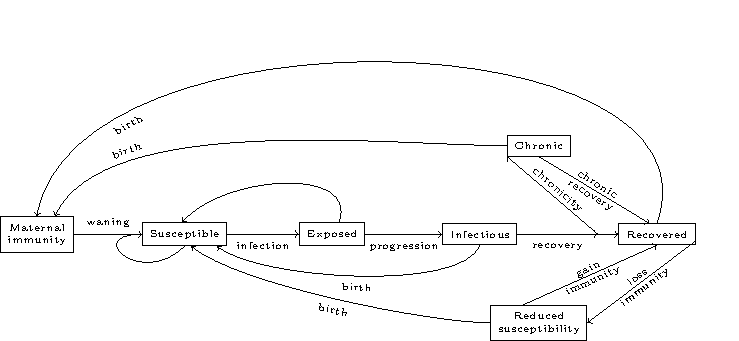
\includegraphics[width=0.9\textwidth]{figure1.pdf}
  \caption{Model diagram (Death from each state is not shown)}
  \label{fig:diagram}
\end{figure}
\end{frame}


\subsection{Data and Analysis}
\begin{frame}
\begin{itemize}
\item Cohort study of about 70 buffaloes.
\item Measurements for antibodies on the three main serotypes have been collected.
\item Implementation of stochastic individual-based model to capture the dynamics of FMD in 
African buffalo.
\item Estimation of corresponding parameters will be implemented using both MLE (point 
estimation) and later Bayesian estimation (distribution estimation).
\item Incorporation of seasonality may be possible.
\end{itemize}
\end{frame}
\end{document}